% \date{2020-Feb-06 10:23:27}
% \documentclass{article}
\title{Temporary}
\author{David Gabriel Corzo Mcmath}
\date{\today}
%%%%%%%%%%%%%%%%%%%%%%%%%%%%%%%%%%%%%%%%%%%%%%%%%%%%%%%%%%%%%%%%%%%%%%%%%%%%%%%%%%%%%%%%%%%%%%%%%%%%%%%%%%%%%%%%%%%%%%%%%%%%%%%%%%%%%%%%%%%%%%%
\usepackage[margin = 1in]{geometry}
\usepackage{graphicx}
\usepackage{fontenc}
\usepackage{pdfpages}
\usepackage[spanish]{babel}
\usepackage{amsmath}
\usepackage{amsthm}
\usepackage[utf8]{inputenc}
\usepackage{enumitem}
\usepackage{mathtools}
\usepackage{import}
\usepackage{xifthen}
\usepackage{pdfpages}
\usepackage{transparent}
\usepackage{color}
\usepackage{fancyhdr}
\usepackage{lipsum}
\usepackage{sectsty}
\usepackage{titlesec}
\usepackage{calc}
\usepackage{lmodern}
\usepackage{xpatch}
\usepackage{blindtext}
\usepackage{bookmark}
\usepackage{fancyhdr}
\usepackage{xcolor}
\usepackage{tikz}
\usepackage{blindtext}
\usepackage{hyperref}
\usepackage{listing}
\usepackage{spverbatim}
\usepackage{fancyvrb}
\usepackage{fvextra}
\usepackage{amssymb}
\usepackage{pifont}
\usepackage{longtable}
\usetikzlibrary{arrows,shapes}
%%%%%%%%%%%%%%%%%%%%%%%%%%%%%%%%%%%%%%%%%%%%%%%%%%%%%%%%%%%%%%%%%%%%%%%%%%%%%%%%%%%%%%%%%%%%%%%%%%%%%%%%%%%%%%%%%%%%%%%%%%%%%%%%%%%%%%%%%%%%%%%






% \begin{document}


%%%%%%%%%%%%%%%%%%%%%%%%%%%%%%%%%%%%%%%%%%%%%%%%%%%%%%%%%%%%%%%%%%%%%%%%%%%%%%%%%%%%%%%%%%%%%%%%
\section{12.1 Sistema tridimensional de coordenadas}
\begin{itemize}
    \item Para localizar un punto en un plano, se necesitan dos números.
    \item Los ejes de coordenadas son perpendiculares entre sí.
    \item En el sistema tridimensional de coordenadas rectangulares, cada punto en el espacio es una terna ordenada.
        \[
          \text{  Espacio:  } \, \mathbb{IR}^3 \{ \quad (x,y,z) \quad \text{  Talque   } \, x,y,z \in \mathbb{IR} .
        \]
        \& 
        \[
          \mathbb{IR}^3 = \mathbb{IR}^2 \times \mathbb{IR}
        \]
    
    \item Sistema 2-D vs. 3-D:
        \begin{figure}[htbp]
            \centering
            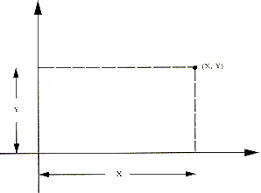
\includegraphics[width=10cm]{./../__Imagenes__/2020-01-07_01.png}
            \caption{}
            \label{}
        \end{figure}
        \begin{figure}[htbp]
            \centering
            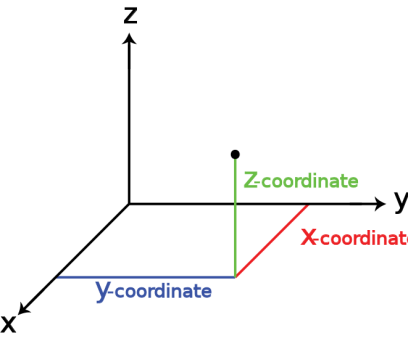
\includegraphics[width=10cm]{./../__Imagenes__/2020-01-07_02.png}
            \caption{}
            \label{}
        \end{figure}
    
    \item Las líneas punteadas se usan para simbolizar las partes debajo, izquierda y detrás.
\end{itemize}



























% \end{document}
